\documentclass[a4paper,10pt]{article}

%A Few Useful Packages
\usepackage{marvosym}
\usepackage{fontspec} 					%for loading fonts
\usepackage{xunicode,xltxtra,url,parskip} 	%other packages for formatting
\RequirePackage{color,graphicx}
\usepackage[usenames,dvipsnames]{xcolor}
\usepackage[big]{layaureo} 				%better formatting of the A4 page
% an alternative to Layaureo can be ** \usepackage{fullpage} **
\usepackage{longtable} 				%for experience
\usepackage{titlesec}					%custom \section
\usepackage{amsmath}
\usepackage{amsfonts}
\usepackage[math]{anttor} % good font! Best with Optima
\usepackage[vlined,linesnumbered,ruled]{algorithm2e}

%Setup hyperref package, and colours for links
\usepackage{hyperref}
\definecolor{linkcolour}{rgb}{0,0.2,0.6}
\hypersetup{colorlinks,breaklinks,urlcolor=linkcolour, linkcolor=linkcolour}

%FONTS
\defaultfontfeatures{Mapping=tex-text}
\setmainfont{Optima}

%CV Sections inspired by: 
%http://stefano.italians.nl/archives/26
\titleformat{\section}{\Large\scshape\raggedright}{}{0em}{}[\titlerule]
\titlespacing{\section}{0pt}{3pt}{3pt}

%tweak page height
%\addtolength{\topmargin}{-.125in}
%\addtolength{\textheight}{0.25in}

%-------------WATERMARK TEST [**not part of a CV**]---------------
\usepackage[absolute]{textpos}

\setlength{\TPHorizModule}{30mm}
\setlength{\TPVertModule}{\TPHorizModule}
\textblockorigin{2mm}{0.65\paperheight}
\setlength{\parindent}{0pt}

\newcommand{\problem}[1]{\section*{Problem #1}}
\newcommand{\answer}{\paragraph{Answer:}}
\newcommand{\proof}{\paragraph{Proof:}}
\newcommand{\qed}{\hfill \ensuremath{\Box}}
\newcommand{\todo}{\textcolor{red}{TODO}{} }

% TODO
%\newcommand{\nless}{\textcolor{red}{TODO!!!}{} }

%--------------------BEGIN DOCUMENT----------------------
\begin{document}

%WATERMARK TEST [**not part of a CV**]---------------
\font\wm=''Baskerville:color=787878'' at 8pt
\font\wmtoday=''Baskerville:color=FF1493'' at 8pt
{\wm 
	\begin{textblock}{1}(0,0)
		\rotatebox{-90}{\parbox{500mm}{
			Typeset by Yang ZHANG with \XeTeX\ on {\wmtoday \today}
		}
	}
	\end{textblock}
}

\pagestyle{empty} % non-numbered pages

\font\fb=''[cmr10]'' %for use with \LaTeX command

%--------------------TITLE-------------
\par{\centering
  {\Large Algorithms and Complexity Analysis}
  \\\vspace{0.5em}
  { Instructed by Yin ZHAO, Spring 2011, Tsinghua University}
  \\\vspace{1.5em}
	{\Huge Solutions for homework 6\vspace{1em}
	}\bigskip\par}

%--------------------SECTIONS-----------------------------------

\problem{17.1-1}

If the set of stack operations included a \texttt{MULTIPUSH} operation, which pushes k items onto the stack,
would the $O(1)$ bound on the amortized cost of stack operations continue to hold?

\answer

No, it won't. Consider the case where \texttt{MULTIPUSH($n$)} and \texttt{MULTIPOP($n$)} appears alternately.

\qed

\problem{17.2-2}

A sequence of $n$ operations is performed on a data structure. The $i$\textsuperscript{th} operation costs $i$ if $i$ is an exact power of 2, and 1 otherwise. 
Use accounting method of analysis to determined the amortized cost per operation.


\answer

Let $c_i$ = cost of $i$\textsuperscript{th} operation.

\begin{equation*}
c_i = \left\{
  \begin{array}{ll}
    i     & \text{if $i$ is an exact power of $2$,}\\
	1 & \text{otherwise.}
  \end{array}
\right.
\end{equation*}

Charge each operation \$3 (amortized cost $\widehat{c_i}$).

\begin{enumerate}
\item If $i$ is not an exact power of $2$, pay \$$1$, and store \$$2$ as credit.
\item If $i$ is an exact power of $2$, pay \$$i$, using stored credit.
\end{enumerate}

Since the amortized cost is \$3 per operation, $\sum_{i=1}^{n}{\widehat{c_i}} = 3n$.

And we have $n$ operations cost:

$$\sum_{i=1}^{n}{c_i} \leq n + \sum_{j=0}^{\lg n}{2^j} = n + (2n - 1) < 3n.$$

Then we have 

$$\sum_{i=1}^{n}{\widehat{c_i}} \geq \sum_{i=1}^{n}{c_i} \Rightarrow 
	\text{credit} = \text{amortized cost} -  \text{actual cost} \geq 0.$$
	
Since the amortized cost of each operation is $O(1)$,
and the amount of credit never goes negative, the total cost of $n$ operations is $O(n)$.

\qed


\problem{17.3-2}

A sequence of $n$ operations is performed on a data structure. The $i$\textsuperscript{th} operation costs $i$ if $i$ is an exact power of 2, and 1 otherwise. 
Use potential method of analysis to determined the amortized cost per operation.


\answer

Consider operation number $i=2^j + k$, where $j$ and $k\geq 0$ are integers and $j$ is chosen as large as possible.
Let the potential function be given by $\phi(D_i) = 2k$. Clearly, this function satisfies the requirements.
There are two cases to consider for the $i$\textsuperscript{th} operation:

If $k=0$ then the actual cost is $i$ and the amortized cost is given by:

\begin{eqnarray*}
\widehat{c_i} &=& c_i + \phi(D_i) - \phi(D_{i-1})\\
&=&i + 0 - 2\times(2^j - 1 - 2^{j-1})\\
&=& i - (2\times(2^j - 2^{j-1}) -2)\\
&=& i  - (2^j \times (2 - 1) - 2)\\
&=& i - i + 2\\
&=& 2.
\end{eqnarray*}

Otherwise the actual cost will be $1$ and we find that

\begin{eqnarray*}
\widehat{c_i} &=& c_i + \phi(D_i) - \phi(D_{i-1})\\
&=&1 + 2k - 2(k - 1)\\
&=& 3.
\end{eqnarray*}

\qed

\problem{17.3-6}

Show how to implement a queue with two ordinary stacks so that the amortized cost of each \texttt{ENQUEUE} and each \texttt{DEQUEUE} operation is $O(1)$.

\answer

Name the two stacks as \texttt{S\_in} and \texttt{S\_out}. The algorithm is given below:

\begin{algorithm}[H]
\caption{\texttt{ENQUEUE}$(e)$}
\texttt{STACK-PUSH}(\texttt{S\_in}, $e$)
\end{algorithm}

\begin{algorithm}[H]
\caption{\texttt{DEQUEUE}$()$}
\While{not \texttt{STACK-EMPTY}(\texttt{S\_in})}{
  $e \leftarrow $\texttt{STACK-POP}(\texttt{S\_in})\\
  \texttt{STACK-PUSH}(\texttt{S\_out}, e)
}
\Return \texttt{STACK-POP}(\texttt{S\_out})
\end{algorithm}

For each element, it is operated in the sequence: \texttt{STACK-PUSH}, \texttt{STACK-POP}, 
\texttt{STACK-PUSH}, \texttt{STACK-POP}, which has $O(1)$ cost.

\qed

\problem{19.2-2}

Show the binomial heap that results when a node with key 24 is inserted into the binomial heap shown in Figure 19.7(d).

\answer

\begin{center}
  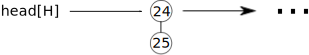
\includegraphics[width=300pt]{sol6-fig1.pdf}
\end{center}

\qed


\end{document}


